%-------------------------------------------------------------------------------
% TEMPLATE FOR ITU HWs and Assignments
% (c) Javad Ibrahimli, 2023

% This is a template for a HWs document, created by JAVAD IBRAHIMLI.
% All rights are reserved. 
%------------------------------------------------------------------------------- 


% ------------------ DOCUMENT SETUP ------------------ 
% The document class defines the document type (report) and sets the font size (12pt)
\documentclass[12pt]{report}
\author{Viet-Linh Le-Viet}


% Inputs the Document Packages
% ------------------ PACKAGES ------------------ 
% Packages add extra commands and features to your LaTeX document. 
% In here, some of the most common packages for a thesis document have been added 
% LaTeX's float package
\usepackage{float}

% LaTeX's color package
\usepackage{color}

% LaTeX's Caption and subcaption packages
\usepackage[format=plain,font=footnotesize,labelfont=bf]{caption}
\usepackage{subcaption}

% The graphicx package provides graphics support for adding pictures.
\usepackage{graphicx}

% Longtable allows you to write tables that continue to the next page.
\usepackage{longtable}

% The geometry packages defines the page layout (page dimensions, margins, etc)
\usepackage[a4paper, lmargin=2.5cm, rmargin=2.5cm, tmargin=2.5cm, bmargin=2.5cm]{geometry}

% Defines the Font of the document, e.g. Arimo font (Check Fonts here: https://tug.org/FontCatalogue/)
% \usepackage[sfdefault]{arimo}
\renewcommand*\ttdefault{cmvtt}
\renewcommand*\familydefault{\ttdefault} %% Only if the base font of the document is to be typewriter style
\usepackage[OT1]{fontenc}

% Font encoding
% \usepackage[T1]{fontenc}

% This package allows the user to specify the input encoding
\usepackage[utf8]{inputenc}

% This package allows you to add empty pages
\usepackage{emptypage}

% Allows inputs to be imported from a directory
\usepackage{import}

% Provides control over the typography of the Table of Contents, List of Figures and List of Tables
\usepackage{tocloft}

% The setspace package controls the line spacing properties.
\usepackage{setspace}

% Allows the customization of Latex's title styles
\usepackage{titlesec}

% Allows the customization of Latex's table of contents title styles
\usepackage{titletoc}

% The package provides functions that offer alternative ways of implementing some LATEX kernel commands
\usepackage{etoolbox}

% Provides extensive facilities for constructing and controlling headers and footers
\usepackage{fancyhdr} 

% Typographical extensions, namely character protrusion, font expansion, adjustment 
%of interword spacing and additional kerning
\usepackage{microtype}

% Manages hyperlinks 
\usepackage[colorlinks=true,linkcolor=black,urlcolor=black,citecolor=black]{hyperref}

% Generates PDF bookmarks
\usepackage{bookmark}

% Add color to Tables
\usepackage[table,xcdraw]{xcolor}


% Acronym Package
\usepackage[acronym]{glossaries}



% Change font size
\usepackage{relsize}

% Blindtext (only for template)
\usepackage{blindtext}

\usepackage{nicefrac, xfrac}


% Controls how many subsections the document can take
%  and how many of those will get put into the contents pages.
\setcounter{secnumdepth}{3}
\setcounter{tocdepth}{3}

% Line Spacing
\setstretch{1.5}


% Places a dot after Chapter/Section/Subsection number in Table of Contents
\renewcommand{\cftchapaftersnum}{.}
\renewcommand{\cftsecaftersnum}{.}
\renewcommand{\cftsubsecaftersnum}{.}

%  Customize Dot spacing in Table of Contents/List of Figures/Tables
\renewcommand{\cftdotsep}{0.3}


% Line Break Properties
\tolerance=1
\emergencystretch=\maxdimen
\hyphenpenalty=10000
\hbadness=10000


% Formatting Table of Contents/Lists titles
\renewcommand{\contentsname}{\bfseries\LARGE{CONTENTS}}
\renewcommand{\listfigurename}{\bfseries\LARGE{LIST OF FIGURES}}

% Signature Line for the declaration
\newbox\namebox
\newdimen\signboxdim

\def\signature#1{%
    \setbox\namebox=\hbox{#1}
    \signboxdim=\dimexpr(\wd\namebox+3cm)
    \parbox[t]{\signboxdim}{%
        \centering
            \hrulefill\\    % for a line
            #1
        \par}%
    }

% Title Formatting customization
\titleformat{\chapter}{\normalfont\bfseries\LARGE}{\thechapter.}{1em}{\MakeUppercase}

\titleformat{\section}{\normalfont\bfseries\large}{\thesection.}{1em}{\MakeUppercase}
\titlespacing*{\section} {0pt} {0pt} {15pt} % left, before, after

\titleformat{\subsection}{\normalfont\bfseries\large}{\thesubsection.}{1em}{}
\titlespacing*{\subsection} {0pt} {15pt} {15pt}

\titleformat{\subsubsection}{\normalfont\bfseries\large}{\thesubsubsection.}{1em}{}
\titlespacing*{\subsubsection} {0pt} {10pt} {10pt}


% HEADER AND FOOTER
\pagestyle{fancy}  % Set Page Style (Header and Footer Style)
% \fancyhf{}  % Clears the header and footer (from the default info)

% Header and footer
\setlength{\headheight}{15pt}
\lhead{Viet-Linh Le-Viet}
\rhead{Homework 2}
\cfoot{\thepage}

% Change figure numbering per section
\numberwithin{figure}{chapter}

%Acronym entries
% \makeglossaries
% \newacronym{US}{US}{Ultrasound}



%  -------------------------------------------------
%  --------- The document starts from here --------- 
%  -------------------------------------------------

\begin{document}


% ------------------  TITLE PAGE -------------------
\begin{titlepage}
\begin{center}

    
    {\relscale{1.90}\textbf{VNU University of Engineering and Technology\\}}
    % UCL IMAGE
    \vspace*{1.0cm}
    \makebox[\textwidth]{
\includegraphics[width=0.2\paperwidth]{img/uet.png}}

    \vspace{0.5cm}
    {\relscale{2.00}\textbf{Image Processing\\}}
    \vspace{0.3cm}
    {\relscale{1.35}\textbf{INT2214 22\\}}
    \vspace{1.4cm}
    
    {\relscale{2.00}{HOMEWORK NO.2}}\\
    %\vspace{0.1cm}
    By\\
    %\vspace{0.1cm}
    Viet-Linh Le-Viet \\ 21020644\\
    \vspace{0.9cm}
    {\begin{singlespace}Course given by:\\\end{singlespace}}
    {\begin{singlespace} Le Thanh Ha\\
    Le Cong Thuong\\\end{singlespace}}


\end{center}
{\vfill{
 \begin{center}
  \today\\
 \end{center}
}\par
}
\end{titlepage}

\tableofcontents

\newpage
% -------------------  OBJECTIVES  ---------------------
\chapter{Image Filtering}
\newpage
\section{Image Padding}
\subsection{Implementation}
\begin{figure} [!h]
    \centering
    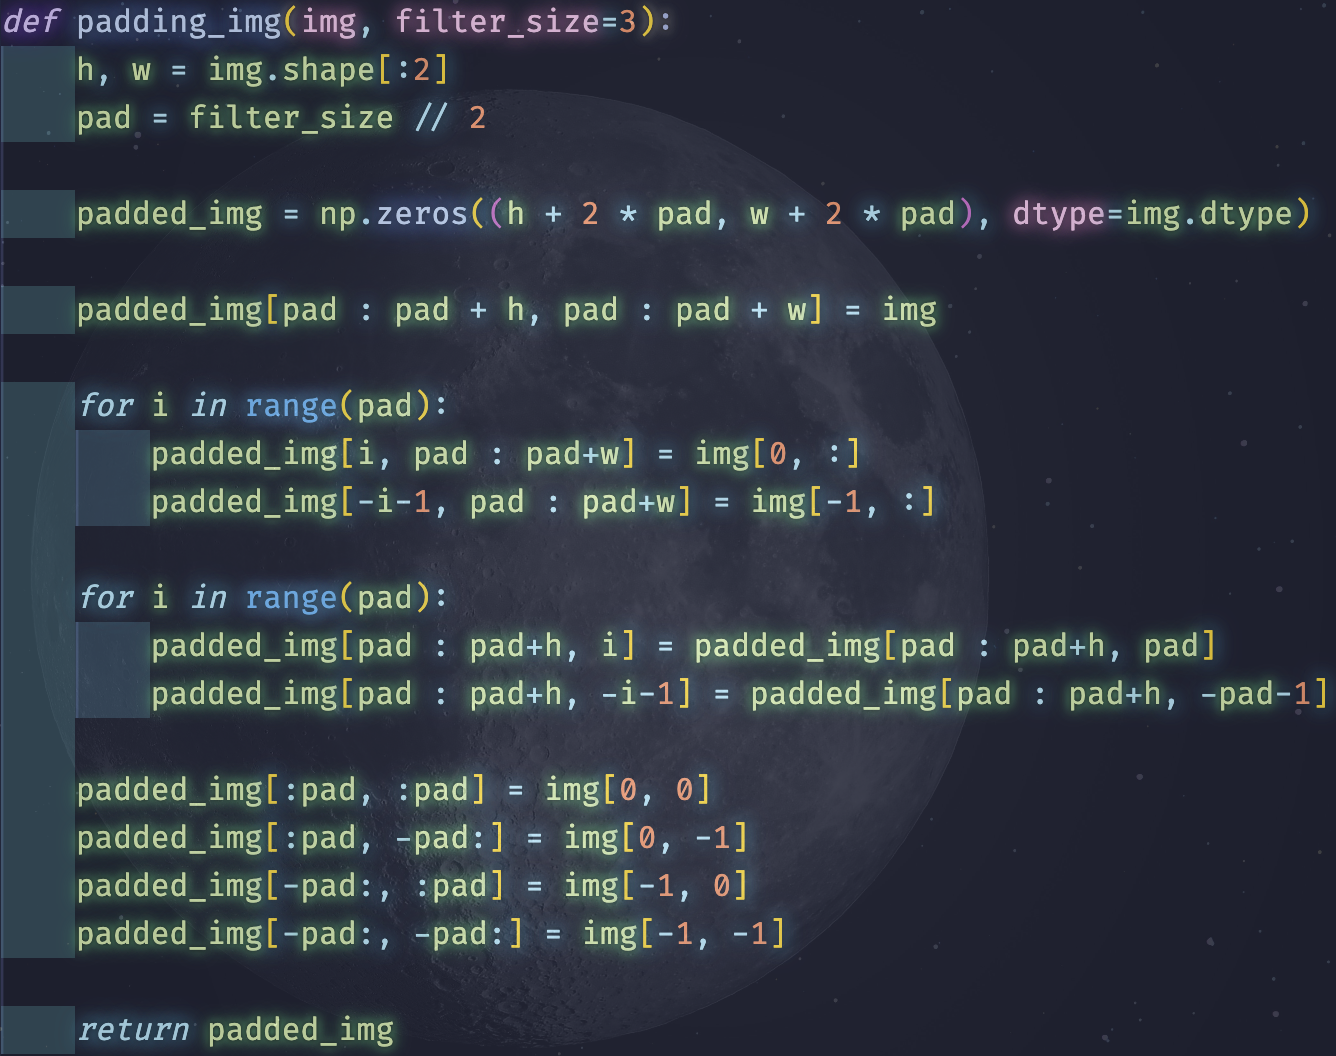
\includegraphics[width=1\textwidth]{img/code/pad.png}
    \caption{Image Padding Function}
\end{figure}

\newpage
\section{Mean Filter}
\subsection{Implementation}
\begin{figure} [!h]
    \centering
    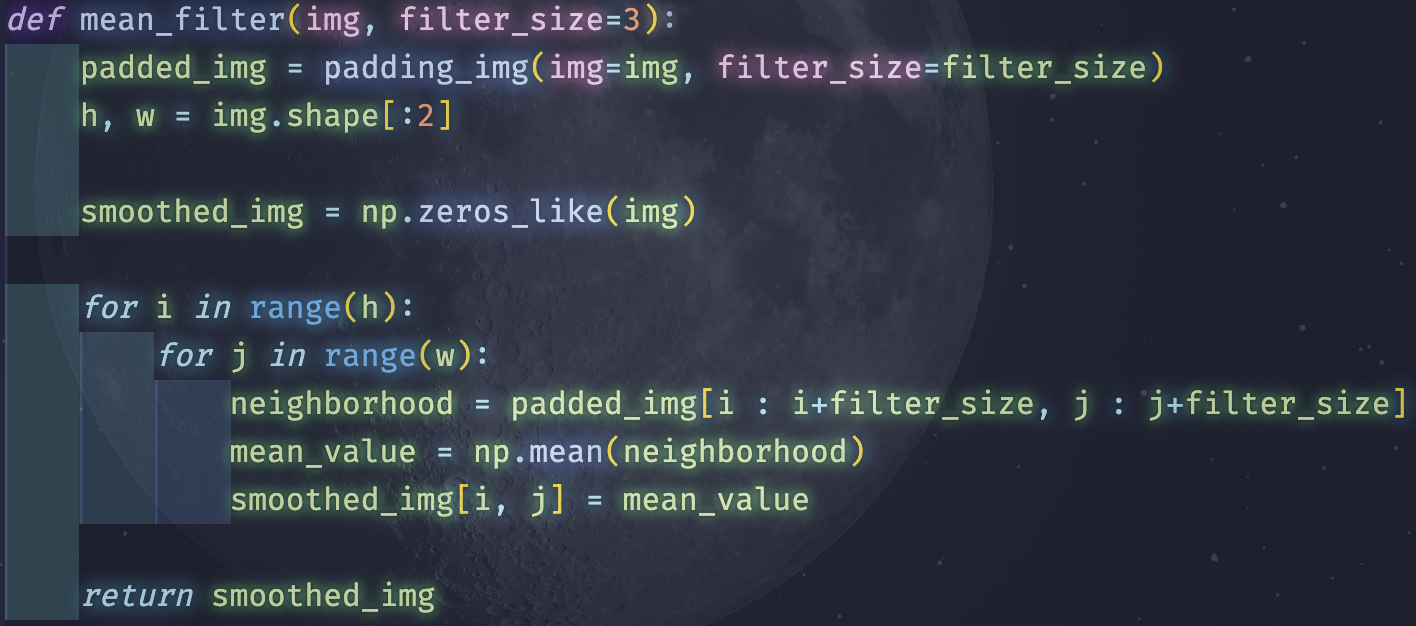
\includegraphics[width=1\textwidth]{img/code/mean.png}
    \caption{Mean Filter Function}
\end{figure}

\subsection{Results}
\begin{figure} [!h]
    \centering
    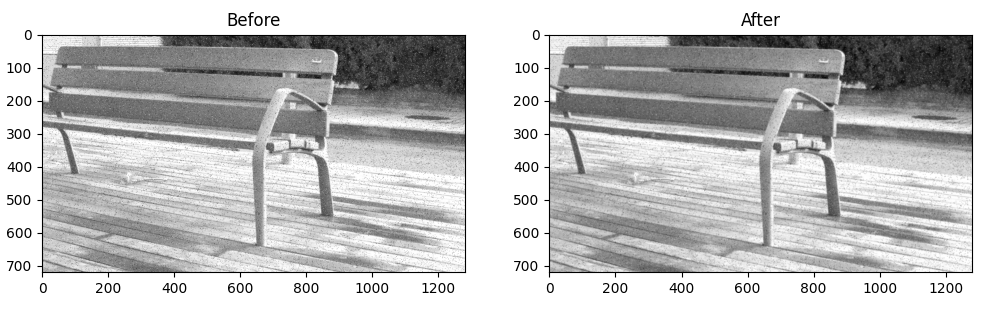
\includegraphics[width=1\textwidth]{img/mean_smoothed.png}
    \caption{Mean Smoothed Image}
\end{figure}

\newpage
\section{Median Filter}
\subsection{Implementation}
\begin{figure} [!h]
    \centering
    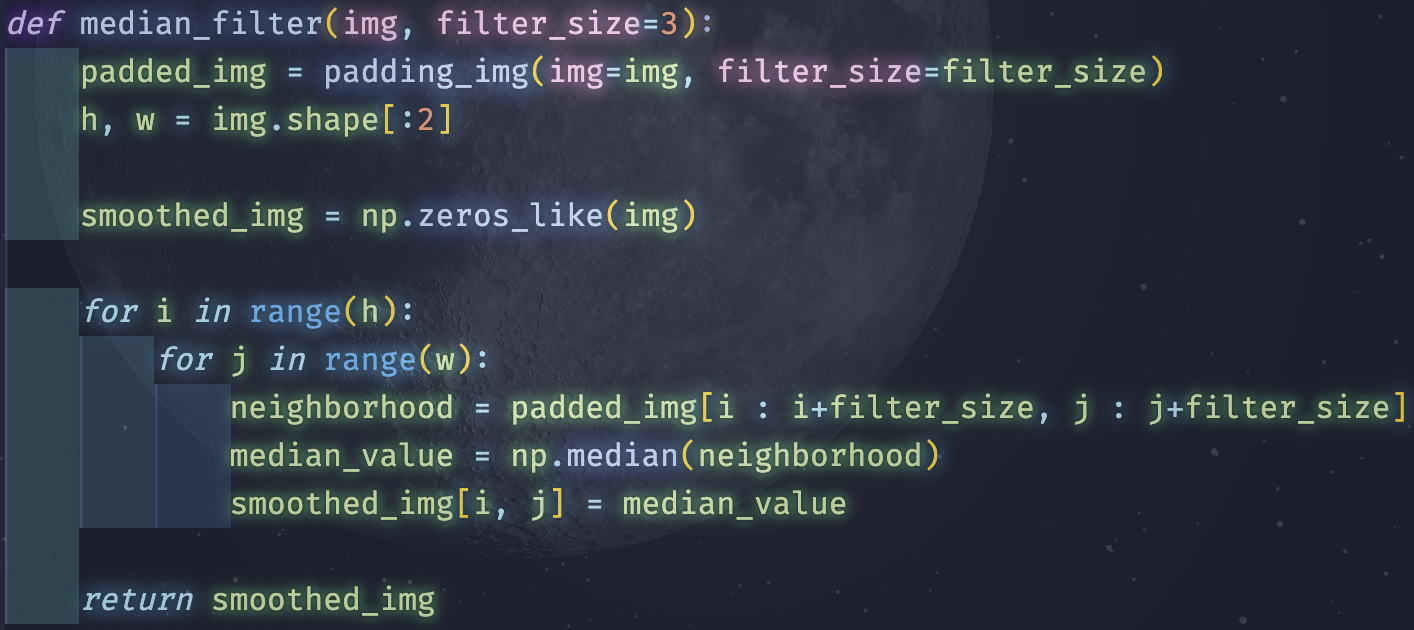
\includegraphics[width=1\textwidth]{img/code/median.png}
    \caption{Median Filter Function}
\end{figure}

\subsection{Results}
\begin{figure} [!h]
    \centering
    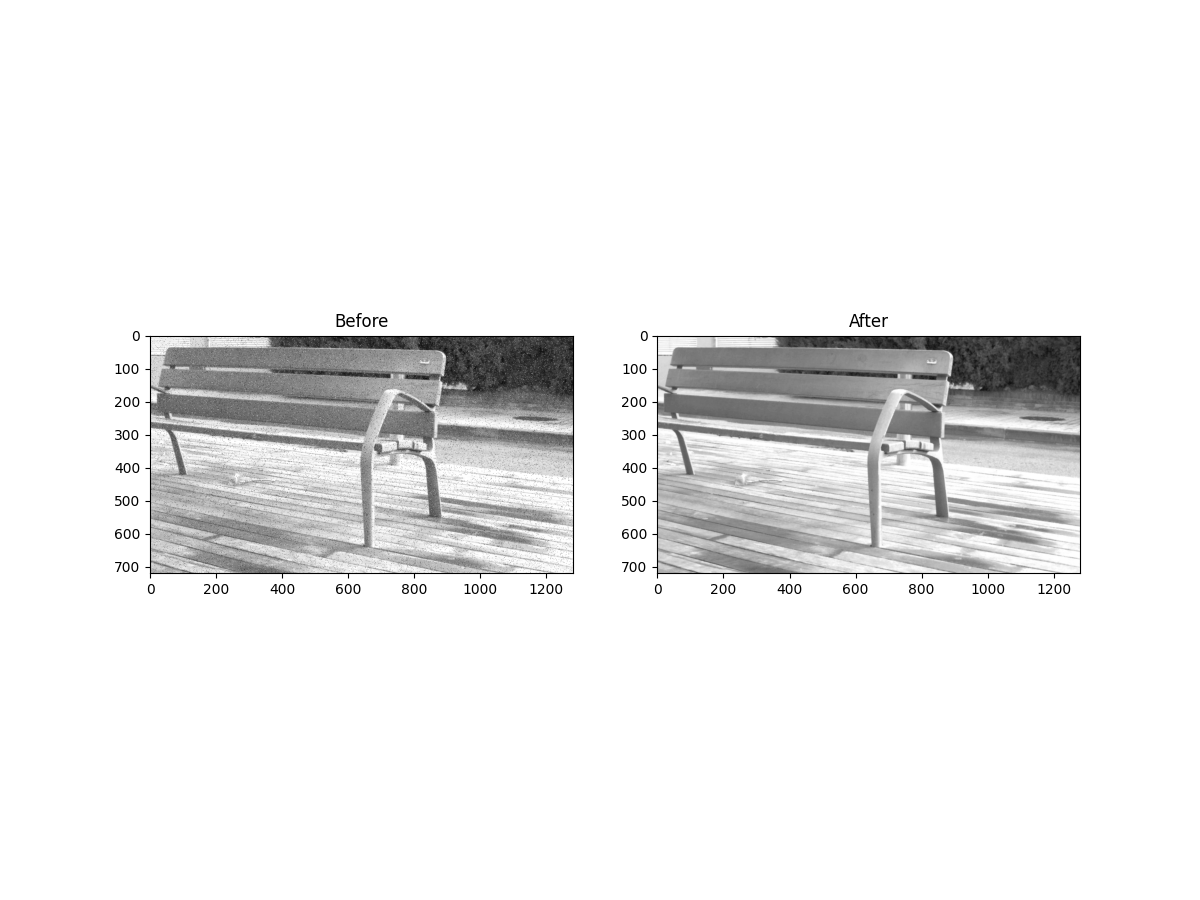
\includegraphics[width=1\textwidth]{img/median_smoothed.png}
    \caption{Median Smoothed Image}
\end{figure} % Section/Chapter entries can be done in the Main.tex file or in a  
                       % separate tex file for longer and more complex documents


% -------------------  RESULTS  ---------------------
\chapter{Fourier Transform}
\newpage
\section{1D Fourier Transform}
\subsection{Implementation}
\begin{figure} [!h]
    \centering
    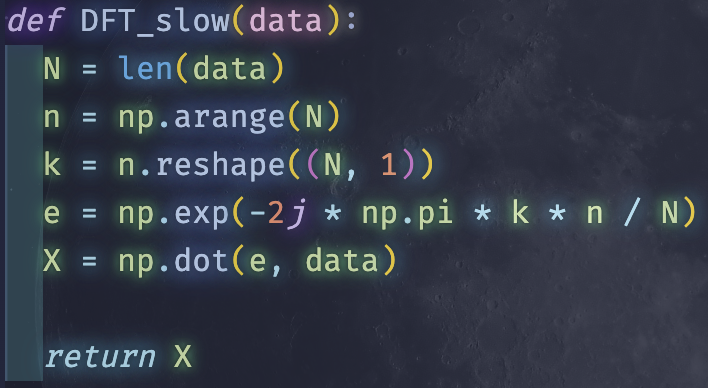
\includegraphics[width=1\textwidth]{img/code/1D.png}
    \caption{1D DFT Function}
\end{figure}


\newpage
\section{2D Fourier Transform}
\subsection{Implementation}
\begin{figure} [!h]
    \centering
    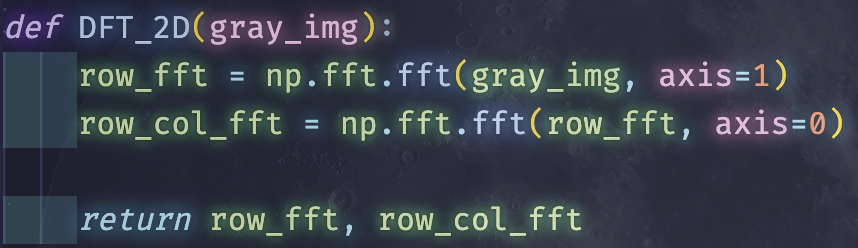
\includegraphics[width=1\textwidth]{img/code/2D.png}
    \caption{2D DFT Function}
\end{figure}

\subsection{Results}
\begin{figure} [!h]
    \centering
    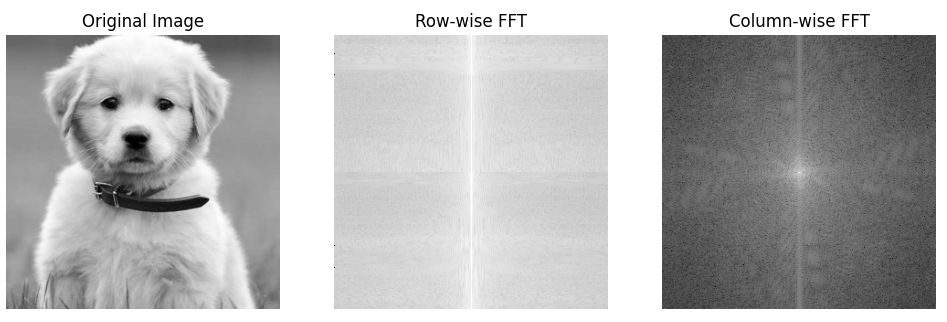
\includegraphics[width=1\textwidth]{img/DFT_2D.png}
    \caption{Output for 2D DFT Exercise}
\end{figure}


\newpage
\section{Frequency Removal Procedure}
\subsection{Implementation}
\begin{figure} [!h]
    \centering
    \includegraphics[width=0.75\textwidth]{img/code/freq.png}
    \caption{Frequency Removal Function}
\end{figure}

\subsection{Results}
\begin{figure} [!h]
    \centering
    \includegraphics[width=0.75\textwidth]{img/freq.png}
    \caption{Output for Frequency Removal Exercise}
\end{figure}

\section{Hybrid Image}
\subsection{Implementation}
\begin{figure} [!h]
    \centering
    \includegraphics[width=0.95\textwidth]{img/code/hybrid.png}
    \caption{Hybrid Image Function}
\end{figure}

\subsection{Results}
\begin{figure} [!h]
    \centering
    \includegraphics[width=1\textwidth]{img/hybrid.png}
    \caption{Hybrid image of a woman and a cat}
\end{figure} % Section/Chapter entries can be done in the Main.tex file or in a  
                       % separate tex file for longer and more complex documents

\end{document}
%  -------------------------------------------------
%  --------- The document ends from here ----------- 
%  -------------------------------------------------